\documentclass[abstract=off,10pt,a4paper,bibliography=totocnumbered]{article}
\usepackage[paper=a4paper,left=35mm,right=35mm,top=25mm,bottom=30mm]{geometry}
\usepackage[doublespacing]{setspace}
\usepackage[english]{babel}
\usepackage[utf8]{inputenc}
\usepackage[round]{natbib}
\usepackage{amsmath}
\usepackage{colortbl}
\usepackage{amsfonts}
\usepackage{amssymb}
\usepackage{gensymb}
\usepackage{graphicx}
\usepackage{tikz}
\usepackage{enumerate}
\usepackage{enumitem}
\usepackage{subcaption}
\usepackage{booktabs}
\usepackage[hidelinks]{hyperref}
\usepackage[nameinlink]{cleveref}
% \usepackage{lineno}
\usepackage{multirow}
\usepackage{arydshln}
% \usepackage[nomarkers, nolists]{endfloat}
\usepackage[flushleft]{threeparttable}
\usepackage{pdflscape}

%------------------------------------------------------------------------------
%	Some Styling
%------------------------------------------------------------------------------
% Creating some TikZ styles
\tikzset{
  nonterminal/.style = {rectangle
    , minimum size = 6mm
    , very thick
    , draw = black!
  }
}

% Changing the style of captions in figures etc.
\captionsetup{labelfont=bf, format=plain, font=small}

% For supplementary material
\newcommand{\beginappendix}{%
  \setcounter{table}{0}
  \renewcommand{\thetable}{S\arabic{table}}%
  \setcounter{figure}{0}
  \renewcommand{\thefigure}{S\arabic{figure}}%
  \setcounter{equation}{0}
  \renewcommand{\theequation}{Equation S\arabic{equation}}%
  \setcounter{section}{0}
  \renewcommand{\thesection}{A.\arabic{section}}%
}

%------------------------------------------------------------------------------
%	Titlepage: Header
%------------------------------------------------------------------------------
\title{\textbf{Appendix}\\ Dispersing through Seasonal Landscapes}

% List of Authors
\author{
  David D. Hofmann\textsuperscript{1,2,\S} \and
  Dominik M. Behr\textsuperscript{1,2} \and
  John W. McNutt\textsuperscript{2} \and
  Arpat Ozgul\textsuperscript{1} \and
  Gabriele Cozzi\textsuperscript{1,2}
}

% Reduce spacing between authors
\makeatletter
\def\and{%
  \end{tabular}%
  \hskip -0.5em \@plus.17fil\relax
  \begin{tabular}[t]{c}}
\makeatother

% Current Date
% \date{\today}

% And here the masterpiece begins
\begin{document}

% Change page numbering
\pagenumbering{gobble}

% Required to be able to cite
\bibliographystyle{apalike}

% Create Titlepage
\maketitle

%------------------------------------------------------------------------------
%	Titlepage: Additional Info
%------------------------------------------------------------------------------
\begin{flushleft}

 \vspace{0.5cm}

 \textsuperscript{1} Department of Evolutionary Biology and Environmental
 Studies, University of Zurich, Winterthurerstarsse 190, 8057 Zurich,
 Switzerland.

 \textsuperscript{2} Botswana Predator Conservation Program, Private Bag 13,
 Maun, Botswana.

 \textsuperscript{\S} Corresponding author (david.hofmann2@uzh.ch)

 \vspace{4cm}

\textbf{Running Title:} Dispersing through Seasonal Landscapes

\vspace{0.5cm}

\textbf{Keywords:} dispersal, simulation, movement, integrated step selection
function, Kavango-Zambezi Transfrontier Conservation Area, landscape
connectivity, Lycaon pictus

\end{flushleft}

%------------------------------------------------------------------------------
%	Main Text
%------------------------------------------------------------------------------
\newpage

% Change page numbering
\pagenumbering{arabic}

% Create linenumbers
% \linenumbers

% Change to appendix counters
\appendix
\beginappendix

%------------------------------------------------------------------------------
%	Appendix S1: Pan Mapping
%------------------------------------------------------------------------------
\newpage
\section{Pan Mapping}
We previously employed a floodmapping algorithm to generate weekly updated
floodmaps, which allowed us to render the seasonal pulsing of the Okavango
Delta. However, due to the coarse resolution of MODIS satellite imagery, based
upon which the floodmaps were derived, prohibited a seasonal representation of
more fine-scaled waterbodies, such as waterpans. In an attempt to overcome this
limitation, we sought out and evaluated alternative satellite products that
would provide better spatial resolution while still retaining sufficient
temporal resolution to meaningfully render seasonal patterns. Candidate products
comprised Landsat 7, Landsat 8, and Sentinel 2 satellite imagery, mainly because
their data is freely accessible, provides a spatial resolution between 10 and 30
meters, and because the satellites have revisit times between 5 and 16 days,
thus allowing to produce monthly updated images. A brief overview of the
characteristics of each product is presented in \Cref{SatelliteData}.

\begin{table}
  \caption{Comparison}
  \label{SatelliteData}
  \begin{tabular}{llll}
             & Availability   & Spatial Resolution & Temporal Resolution                             \\
  Landsat 7  & 1999 - Present & 15-60m             & Every 16th day                                  \\
  Landsat 8  & 2013 - Present & 15-100m            & Every 16th day                                  \\
  Sentinel 2 & 2015 - Present & 10-60m             & Every 10th day / every 5th day since March 2017
  \end{tabular}
\end{table}

While Landsat 7's temporal availability would have aligned with the time window
during which we collected GPS data on dispersing wild dogs, Landsat 7's scan
line detector has been failing since May 31 2003, resulting in data gaps between
adjacent tiles, thus rendering this product unusable for our purposes.

With Landsat 8 and Sentinel 2 imagery remaining as viable candidates, we
prepared a set of training polygons, consisting of the land cover classes
\textit{Dryland}, \textit{Water}, and \textit{Wet Pans}. Although our primary
goal was to detect wet pans, we deliberately added additional classes,
anticipating that their inclusion would facilitate the separation of reflectance
values. Due to the large extent considered and limited time available in the
field, \textit{in situ} collection of training data was unfeasible and we
instead opted for \textit{on-screen selection} of training data. More
specifically, we used Google Earth to digitize areas that were clearly
identifiable as either dryland, water, or wet pan. At the highest zoom level
that is allowed in Google Earth, these categories are visually easy to
distinguish \Cref{PanMapping}. To verify a sharp distinction between wet and dry
pans, we placed several dryland polygons on areas that are seasonally covered by
water \Cref{PanMapping}. Depending on the area of interest, Google Earth
displays high-resolution satellite imagery collected on different dates, so
assigned to each training polygon the date of acquisition of the displayed
satellite image. This later allowed us to train the land cover classifier using
Sentinel 2 or Landsat 8 data imagery acquired on the same dates. This procedure
resulted in xx polygons (xx dryland, xx water, xx dry-pan, and xx wet-pan)
distributed across xx dates.

\begin{figure}[htbp]
 \begin{center}
  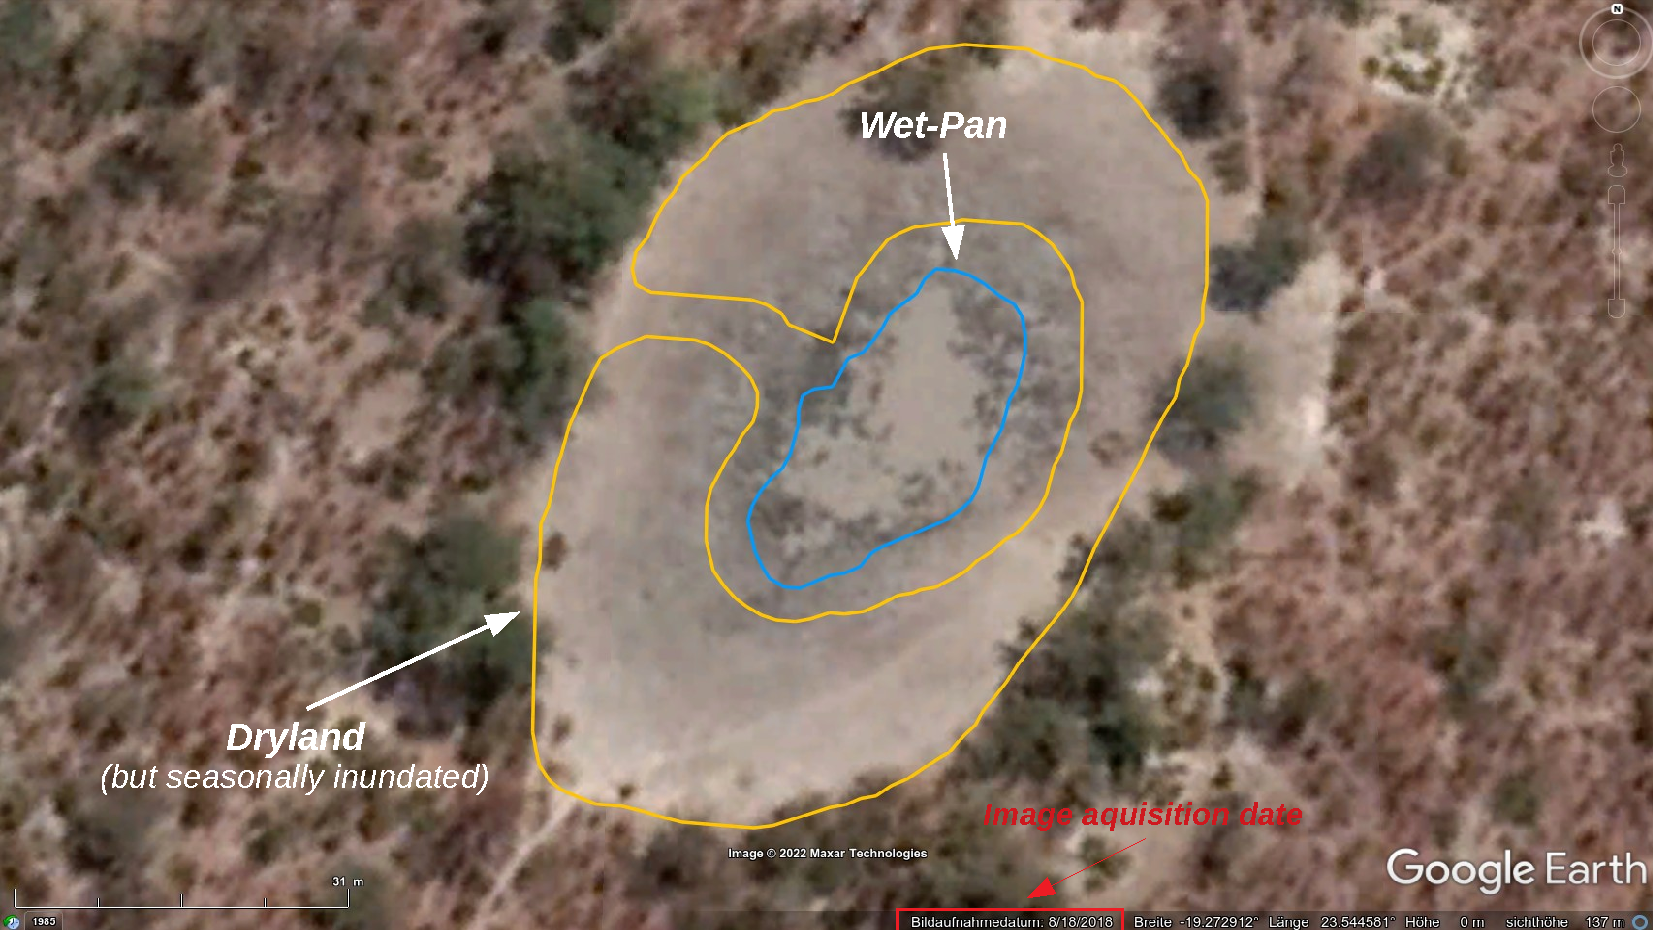
\includegraphics[width = \textwidth]{99_PanMapping.pdf}
  \caption{Example of a \textit{wet pan} and \textit{dryland} training polygon
  digitized on Google Earth. The extent of water can easily be gauged at this
  zoom level in Google Earth. While the dryland polygon in this case covered an
  area that is seasonally covered by water, other dryland polygons comprised
  areas that are never inundated. However, to ensure reliable differentiation
  between wet and dry pans, we included several dryland polygons located in dry
  pans.}
  \label{PanMapping}
 \end{center}
\end{figure}

% Download of data and preprocessing of satellite data (atmospheric correction,
% cloud cover etc.). Computation of indices.

To train a land-cover classifier, we selected 3'000 training points within the
digitized training polygons following a stratified equal random sampling scheme
\citep{Shetty.2021}. That is, we ensured that a total of 1'000 random points per
land cover category were generated. This was necessary to ensure that pans,
which only accounted for a very small fraction of the study area, were
sufficiently well sampled. In fact, stratified equal random sampling has been
shown to provide good class-level accuracy for minority classes, so we deemed
this approach suitable for our purposes. At each generated random point we then
extracted reflectance values of Sentinel 2 and Landsat 8 bands that temporally
aligned with the date assigned to the respective random point
\Cref{Reflectances}. For instance, if a random point fell into a polygon that
was digitized using a Google Earth image generated on Dec 18 2018, we extracted
values from the Sentinel 2 and Landsat 8 composite for December 2018. Using the
extracted values, we parametrized a Random Forest (RF) classification model.

\begin{figure}[htbp]
 \begin{center}
  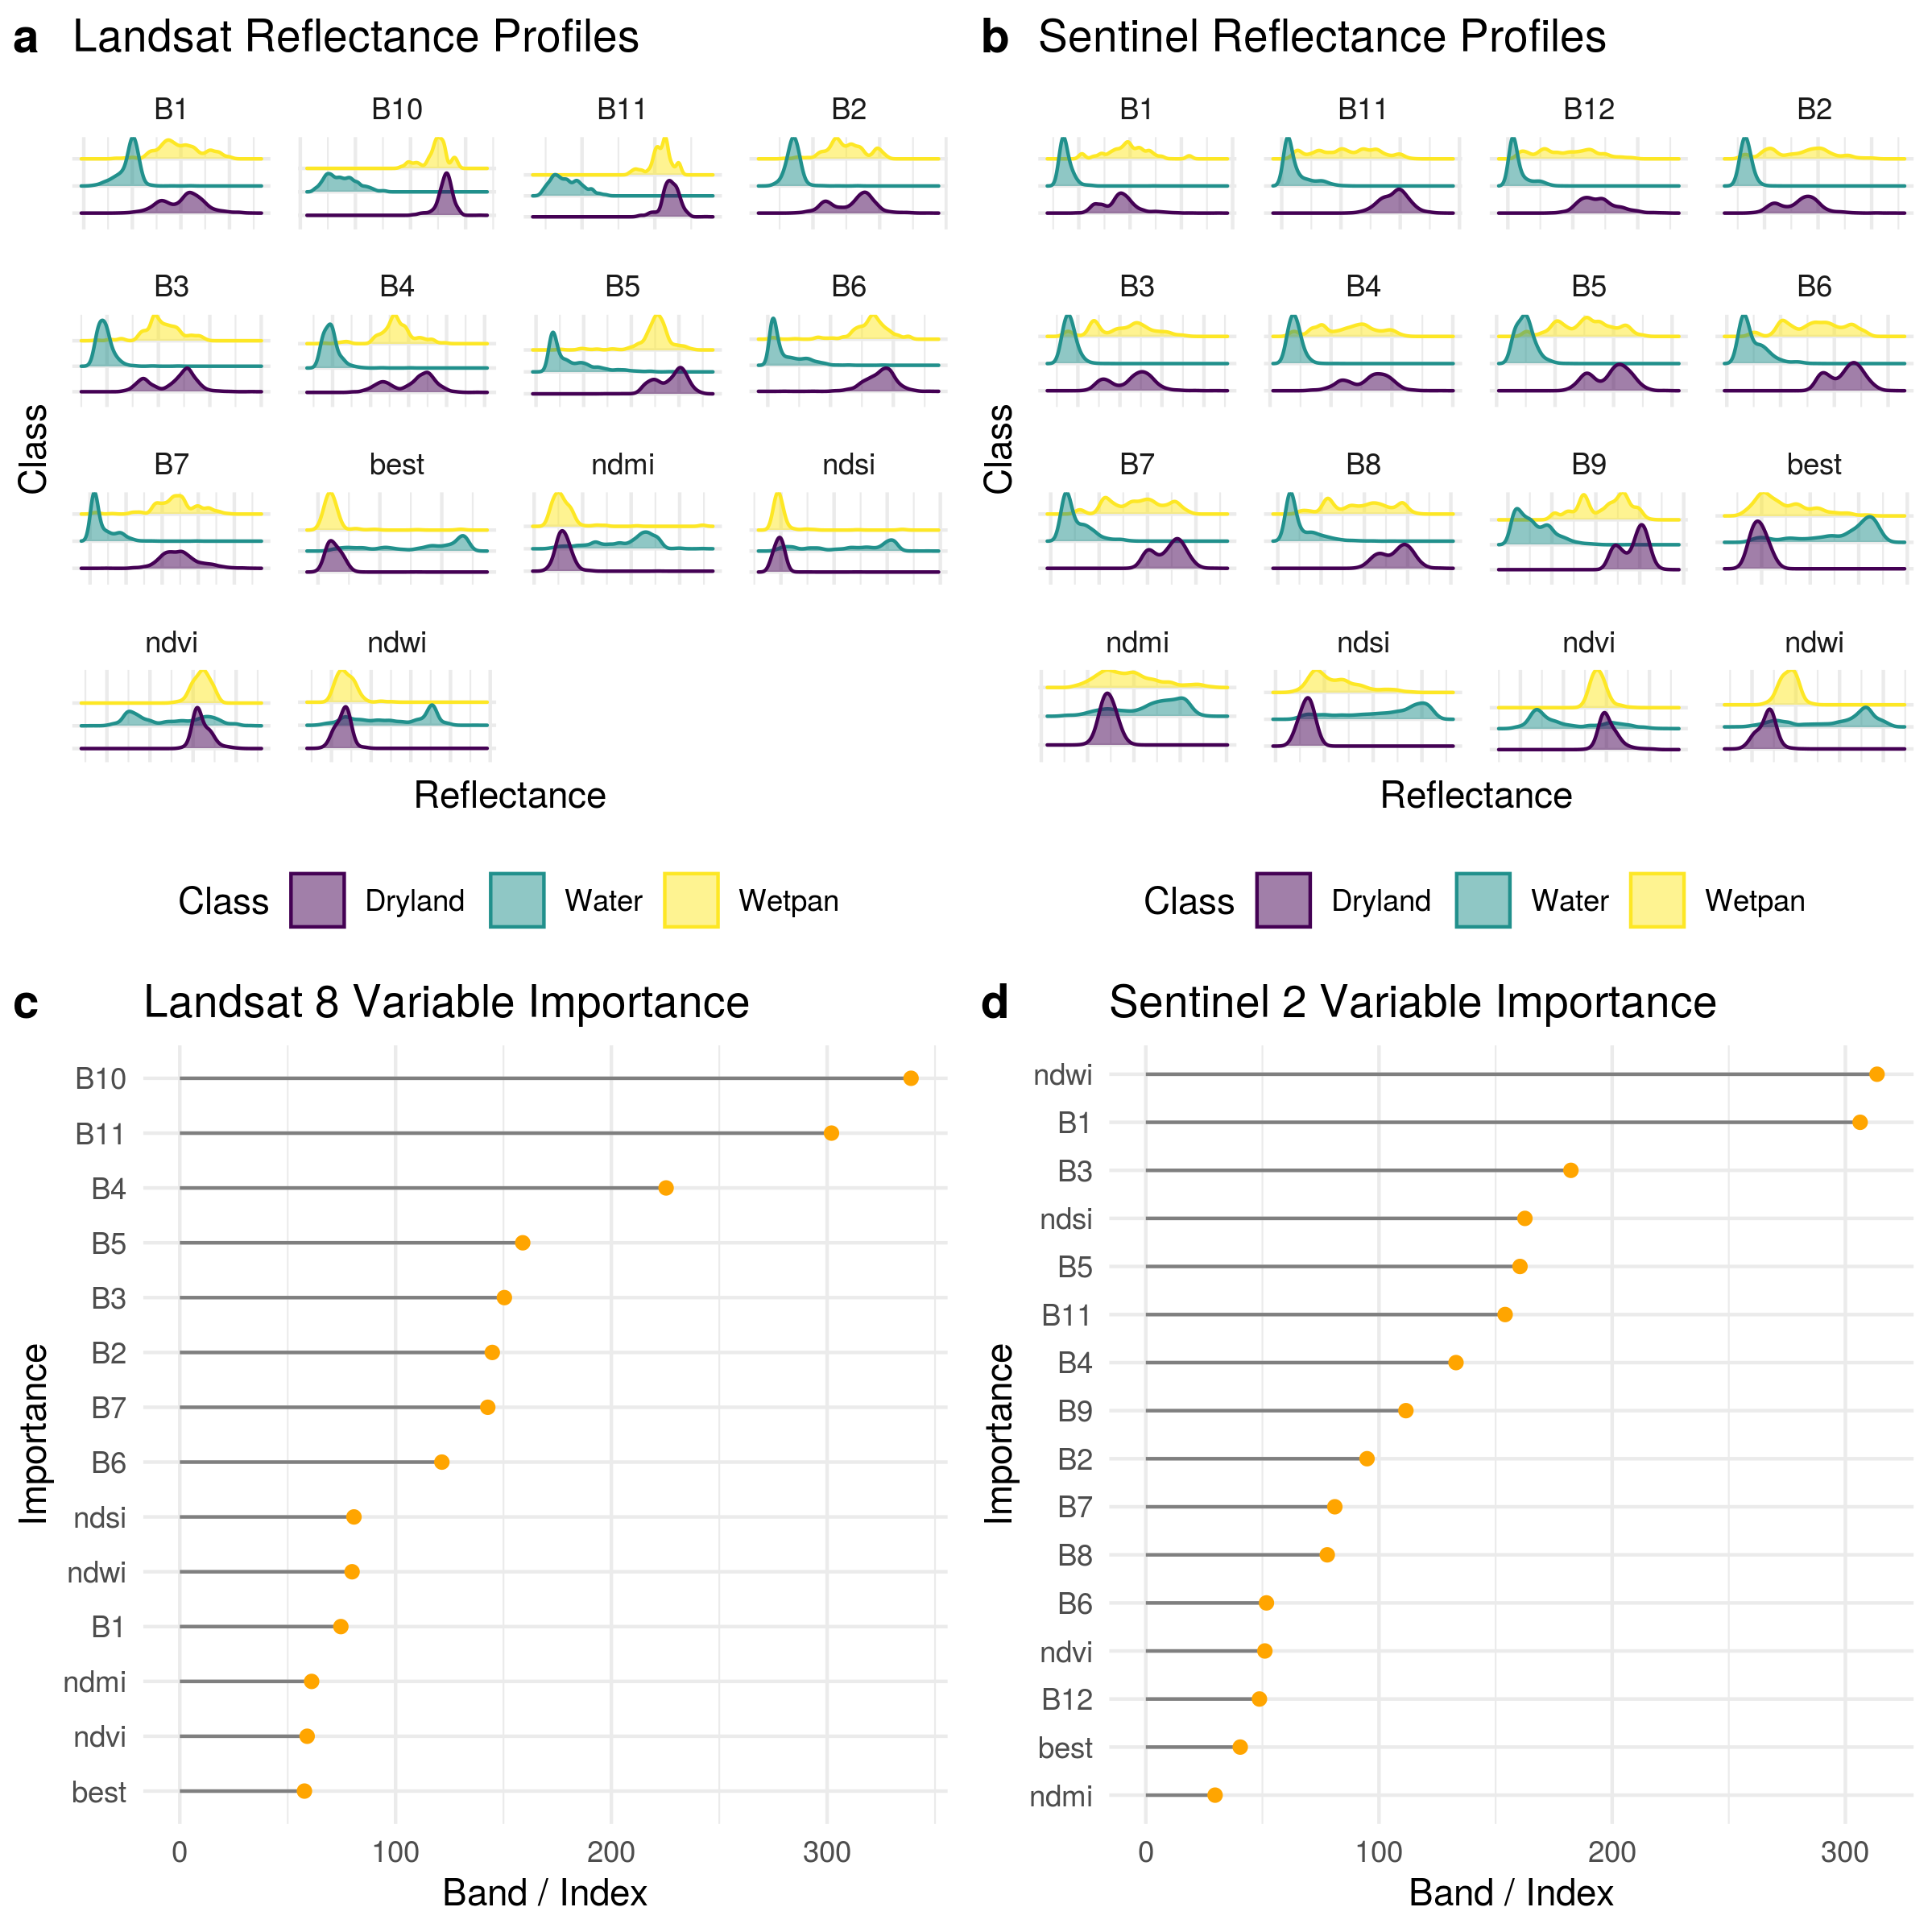
\includegraphics[width = \textwidth]{99_Reflectances.png}
  \caption{}
  \label{Reflectances}
 \end{center}
\end{figure}

To validate the predictive power of the RF classifier, we employed 5-fold
cross-validation. For this, we split the data into 5 groups and repeatedly
fitted the RF model using 80\% of the data while predicting land cover
categories on the remaining 20\%. We then contrasted predictions with true
classes and computed confusion matrices to obtain estimates of the classifier's
specificity, sensitivity, and overall accuracy. The results from this validation
show that the RF classifier achieves very high overall accuracy, for both
Landsat 8 and Sentinel 2 imagery \Cref{ClassificationValidation}.

\begin{figure}[htbp]
 \begin{center}
  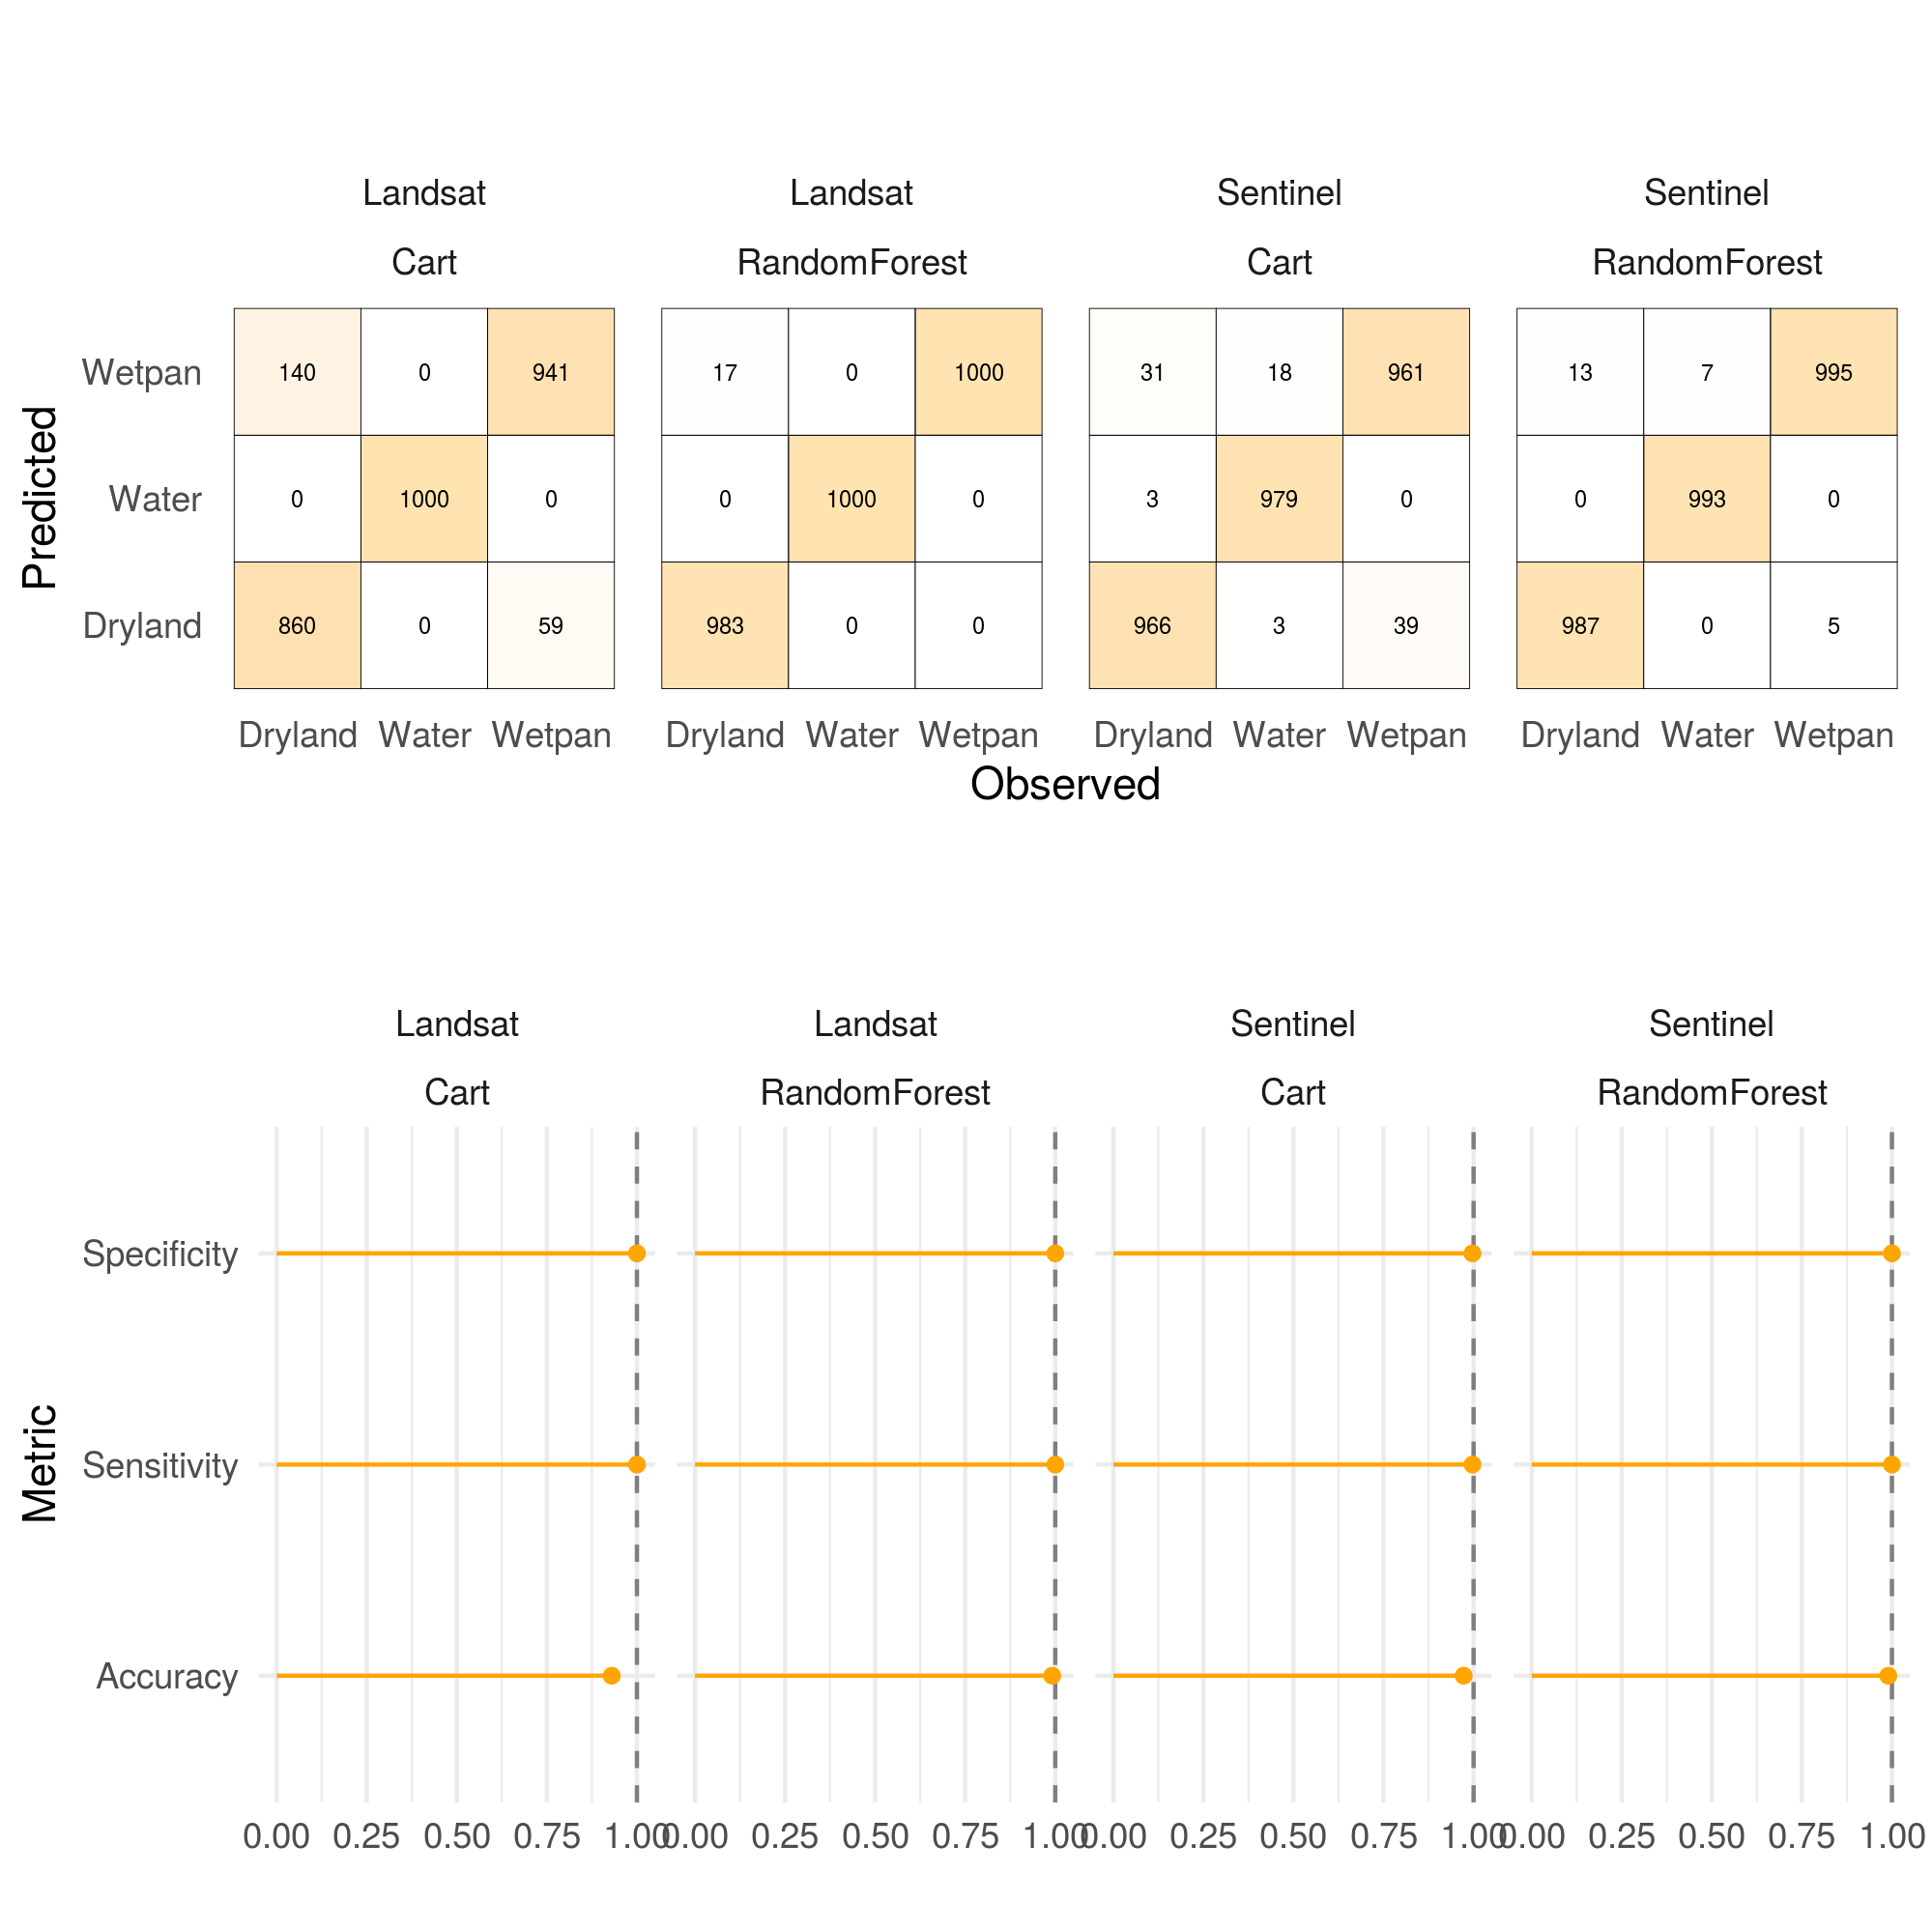
\includegraphics[width = \textwidth]{99_ClassificationValidation.png}
  \caption{}
  \label{ClassificationValidation}
 \end{center}
\end{figure}

While both Landsat 8 and Sentinel provided very good results, we opted for
Sentinel 2 data, mainly due Sentinel 2's better temporal coverage and marginally
higher resolution, which we thought was crucial for pan detection. To download
satellite imagery of interest, we first generated a spatio-temporal moving
window comprising all GPS locations from dispersing wild dogs of a given month,
buffered by 100km. We checked for intersections of each month's moving window
with Sentinel 2's tile-grid and determined the tiles to be downloaded for every
month. For the intersecting tiles, we then downloaded all available Sentinel 2
images falling into the respective month. Download and pre-processing of all
Sentinel 2 images was achieved using the \textsf{sen2r} package in R. While
atmospherically corrected Sentinel 2 data is currently being fed into ESA's
database, a large portion has not yet been processed from level 1C (top of the
atmosphere, TOA) to level 2C (bottom of the atmosphere, BOA). Thus, whenever
level 2C data was not available, we downloaded level 1C data and pre-processed
the imagery into level 2C using sen2cor \citep{MainKnorn.2017}, again invoked
through \textsf{sen2r}.

\newpage
\begingroup
\singlespacing
\bibliography{Literatur}
\endgroup

\end{document}
